\documentclass{tufte-handout}

%\geometry{showframe}% for debugging purposes -- displays the margins
\usepackage{pdfpages}
\usepackage{amsmath}
\usepackage{natbib}
\usepackage{booktabs}
\usepackage{multicol}
\usepackage[version=4]{mhchem} 

\bibfont{\small} % Doesn't see to work...
\usepackage{graphicx}

\setkeys{Gin}{width=\linewidth,totalheight=\textheight,keepaspectratio}
\graphicspath{{graphics/}}

\newenvironment{itemize*}%
  {\begin{itemize}%
    \setlength{\itemsep}{0pt}%
    \setlength{\parskip}{0pt}}%
  {\end{itemize}}
	
\newenvironment{enumerate*}%
  {\begin{enumerate}%
    \setlength{\itemsep}{0pt}%
    \setlength{\parskip}{0pt}}%
  {\end{enumerate}}
	

\title{The Physics of Soil Particle Size Analysis by Hydrometer %\thanks{Isaac Medina}
}
\author[Marc Los Huertos]{Marc Los Huertos}
%\date{}  % if the \date{} command is left out, the current date will be used

% \SweaveOpts{prefix.string=graphics/plot} % Created a "graphics" subdirectory to 

\setsidenotefont{\color{blue}}

\usepackage{Sweave}
\begin{document}
\Sconcordance{concordance:Physics_Soil_Particle_Size_Analysis.tex:Physics_Soil_Particle_Size_Analysis.Rnw:%
1 38 1 1 0 10 1 1 5 39 1 1 3 1 2 230 1 1 7 10 1 1 8 4 1 1 9 18 0 1 2 20 1 1 4 4 0 1 6 3 0 %
1 2 6 1 1 10 1 2 19 1 1 10 1 1 1 7 1 2 8 1}


\maketitle% this prints the handout title, author, and date
\begin{abstract}
\noindent Soil is usually composed of particles with a mix of sizes where the relative proportion of size classes define the soil texture. As a property of a soil, the texture can determine water relations, bio-availability of nutrients and toxics, and soil biogeochemistry. Soil texture can be determined using qualitative or quantitative methods that might be employed in the field or in the laboratory, respectively. Classes are distinguished in the field and the class is then used to determine crop suitability and to approximate the soils responses to environmental and management conditions such as drought, fertility, or calcium (lime) requirements.
\end{abstract}

%\printclassoptions

% Setting up the margins, etc for R

\section{Outline and Outcomes}
This handout describes how soil samples can be quantitatively analyzed using hydrometer to promote the following skills:

\begin{enumerate}
	\item Understand equations that describe particle size and terminal velocity in a suspension;
	\item Use sedimentation methods to measure density changes in soil suspensions; and
	\item Apply equations to calculate the density and percent of a sample in suspension to calculate the particle sizes of a soil sample. 
\end{enumerate}

\section{Background}

Soils are composed of mineral particles, organic matter, water and air. In general, most of the mass of soil is composed of mineral particles and the size or texture of these particles influence a range of physical and biological processes in soil. In the simplest cases, we can categorize the size of particles into three groups: Sand, silt, and clay. In general, we consider soil to be made up of particles that can pass through a 2 mm sieve, aka No. 10 sieve (Figure \ref{fig:8stainless_sieve}). 

\begin{marginfigure}
	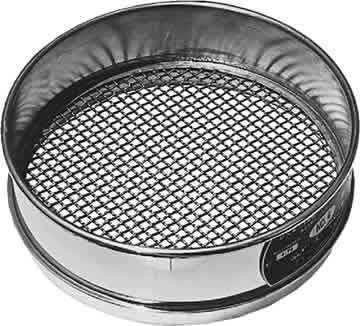
\includegraphics{8stainless_sieve.jpg}
	\caption{Sieves are circular dishes with a mesh bottom. Each sieve type have different mesh sizes, thus can be used to ``split'' soils based on the size of particles, where particles smaller than the mesh fall through and larger particles are retained.}
	\label{fig:8stainless_sieve}
\end{marginfigure}

\begin{table}
		\begin{tabular}{lrr}\hline
Classification 					&  USDA System (Retained by Sieve No.) 		& World Reference Base (Retained by Sieve No.)\\ \hline\hline
			Clay 							& <0.002 mm 							& <0.002 mm \\
			Silt 							& 0.002-0.05 mm 					& 0.002-0.063 mm\\
			Very fine sand		& 0.05-0.10 mm						& 0.063-0.0125 (No. 230) mm\\
			Fine sand 				& 0.10-0.25 mm 						& 0.0125-0.20 (No. 120) mm\\
			Medium sand				& 0.25-0.50 mm (No. 60) 	& 0.20-0.63 mm\\
			Coarse sand 			& 0.50-1.00 mm (No. 35) 	& 0.63-1.25 mm\\
			Very coarse sand	& 1.00-2.00 mm (No. 18)		& 1.25-2.00 mm\\
			Gravel 						& >2.0 mm (No. 10)				& >2.0 mm \\ \hline
		\end{tabular}
\end{table}


There are a number of references that explain various methods to conduct a particle analysis, such as \citep{gee1986particle, day1965particle, beretta2014soil}. For our purpose, we will use the method developed by the ASTM International that capitalizes on the correlation between the size of particles, their terminal velocity, and the density of the suspension \citep{standard2007d422}. 

This handout describes how we can use a hydrometer to measure density of a soil suspension and how this density changes with time. As the density changes, we can use several equations to estimate the proportion of particle sizes. 

\begin{figure}
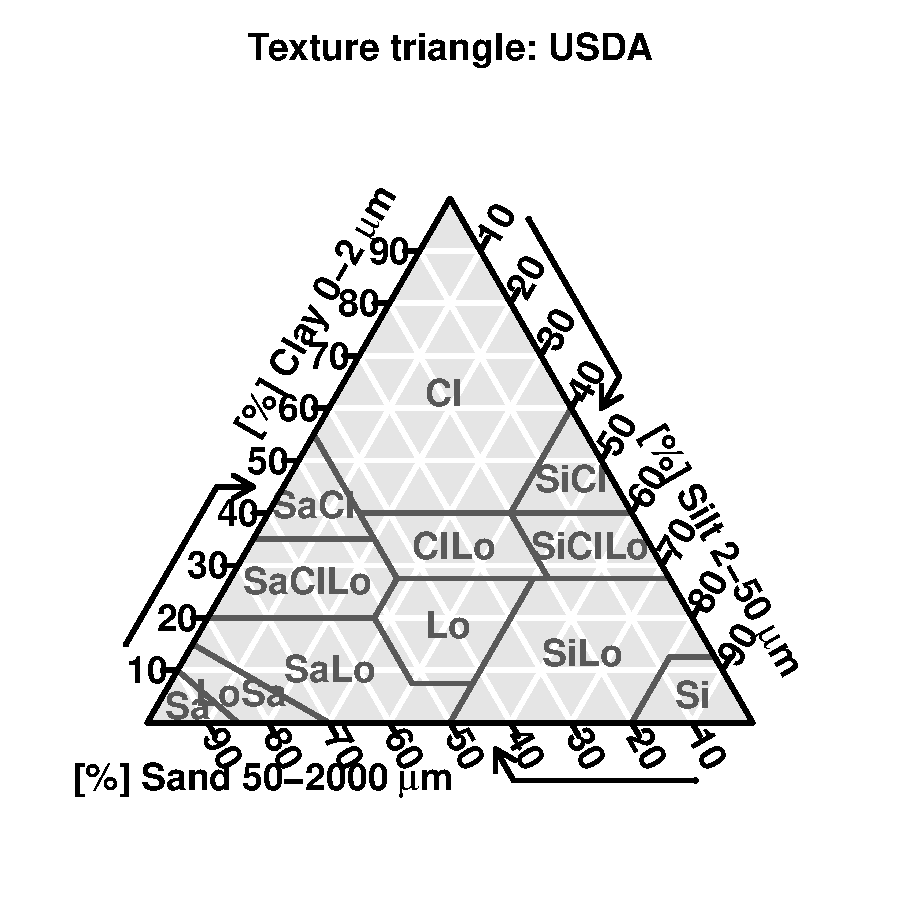
\includegraphics{Physics_Soil_Particle_Size_Analysis-USDATT}
\end{figure}

\subsection{Physics of Particles in Suspension}

The behavior of particles in a suspension is well understood\sidenote{This section is from \citet{hillel1998environmental}.}, where particles are accelerated by the force of gravity, g, which is 9.8 m/sec$^2$. Except in a vacuum, particles experience resistance. This force of resistance, $F_r$, is proportional to the radius and velocity of the particle and the viscosity of the fluid that surrounds it. This was defined by George Stokes in 1851 as

\begin{equation}\label{eq:Fr}
F_r = 6\pi \eta r \nu
\end{equation}

\noindent where r is the radius, 
$\eta$ is the fluid viscosity and 
$\nu$ is the velocity.

The downward force due to gravity, $F_g$, proportional to the volume of the particle, $(4/3)\pi r^3$, and difference in particle and fluid densities, $\rho_p - \rho_f$.\sidenote{suspension, solid, and soil can each be referred to with the subscript of s in soil physics, which is confusing. In addition, is the subscript for fluid referring to pure water or water with particles suspended in it? I will change these equations for p for particle and w for pure water, and f for the fluid with suspended particles.}

\begin{equation}\label{eq:Fg}
F_g = volume \cdot (\rho_p - \rho_f)g = (4/3)\pi r^3(\rho_p - \rho_f)g 
\end{equation}

\noindent where g = acceleration due to gravity. 
As particles accelerate in the water column, they reach a terminal velocity when $F_r = F_g$. Thus, we can set Equations \ref{eq:Fr} and \ref{eq:Fg} equal to each other,

\begin{equation}
6\pi \eta r \nu = (4/3)\pi r^3(\rho_p - \rho_f)g
\end{equation}

\noindent And we can re-arrange the equation for the terminal velocity, $\nu_t$,

\begin{equation}
\nu_t = (2r^2g/(9\eta))(\rho_p - \rho_f)
\end{equation}

\noindent and since the diameter (d) is $2r$, we can substitute in $d$, and obtain 

\begin{equation}\label{eq:mu_t}
\nu_t = (d^2g/(18\eta))(\rho_p - \rho_f)
\end{equation}

\noindent Now if we assume that the terminal velocity of the particle is reached nearly instantaneously, we can calculate the time that a particle travels a vertical distance, h, 

\begin{equation}
\nu_t = h/t
\end{equation}
 
\noindent By substituting the velocity equation into Equation \ref{eq:mu_t} and obtain,

\begin{equation}
h/t = (d^2g/(18\eta))(\rho_p - \rho_f)
\end{equation}

\noindent And finally, by solving for the diameter, or size of particle, we get

\begin{equation}
d = [18h\eta/(tg(\rho_p - \rho_f))]^{1/2}
\end{equation}

\subsection{Assumptions in Applying Stokes' Law}

As we might guess, there are assumptions that must be met for any law in physics. 
Basic assumptions used in applying Stokes' Law to sedimentating soil suspensions are:
 
\begin{enumerate}
	\item Terminal velocity is attained as soon as settling begins,
	\item Fluid flow around the particles is laminar, i.e. no particle exceeds the critical velocity for the onset of turbulence, 
	\item Settling and resistance are entirely due to the viscosity of the fluid (hydrometer or pipet and the sedimentation-cylinder wall may also influence the settling rate),
	\item Particles are rigid, smooth, and spherical (in contrast, clay particles, in particular, may be platy),
	\item The suspension is sufficiently dilute that individual particles do not interfere with one another and each settles independently,  
	\item All particles have the same density. Ordinarily $\rho_p$ (particle density) is considered to be 2.65 or 2.60 Mg m$^{-3}$ (equivalent to g cm$^{-3}$), however it may vary between 2.0 to 3.2 Mg m$^{-3}$, and
	\item Temperature of the water should be constant throughout sedimentation.
\end{enumerate}

Violations of these assumptions reduces the accuracy of the method. However, for our purposes, these inaccuracies should have little influence in the overall results.  

\subsection{Buoyancy: Applying Stokes Law Using a Hydrometer}

As progressively smaller particles drop out of the suspension, the density of the suspension itself declines. So, there are two components to the density of the suspension -- the relative concentration of the particles suspended and the time in which they remain in suspension. Since smaller particles remain in suspension longer, we can combine these parameters, of the density of a solution or suspension and proportion of the particle sizes that remain in suspension, to estimate the particle size distribution. 

We apply the concept of buoyancy to evaluate the density of suspension. Just like the forces of gravity ($F_g$) and resistance ($F_r$), objects in fluids can also be influenced by the force of buoyancy, where Archimedes' principle that a solid suspended in a fluid is buoyed by a force equal to the weight of the fluid displaced by the submerged part of the suspended solid. 

\begin{equation}
F_b = V_f \rho_f g
\end{equation}

\noindent where $F_b$ is the buoyancy force, $V_f$ is the volume of the displace volume, $\rho_f$ is the density of the fluid displaced, and g is the acceleration due to gravity.

The application of simple physical principles allows the relative density, or specific gravity, of the unknown liquid to be calculated from the change in displacement. For example, in soils the specific gravity of a particle can be calculated 

\begin{equation}
GS_p = \rho_p / \rho_w
\end{equation}

\noindent where $GS_p$ is the specific gravity of a particle in water, 
$\rho_p$ is the density of a particle, and
$\rho_w$ is the density of pure water.

%\textbf{NOTE:} Density = Mass / Volume. Specific gravity is the density of a substance divided by the density of water. Since (at standard temperature and pressure) water has a density of 1 gram/cm$^3$, and since all of the units cancel, specific gravity is usually very close to the same value as density (but without any units).

%The specific gravity of water $Gs_w$ of water approximately $\rho_w$. Some algebraic thoughts... $\rho_p$ = $Gs_w$ * $Gs_p$, $\rho_p$ - $\rho_f$ ($Gs_w$ * $Gs_p$) - $Gs_w$

A hydrometer is an instrument that measures the specific gravity (relative density) of liquids---the ratio of the density of the liquid to the density of water. A hydrometer is usually made of glass, and consists of a cylindrical stem and a bulb weighted with mercury or lead shot to make it float upright (Figure \ref{fig:Hydrometer151H}). Operation of the hydrometer is based on Archimedes' principle that a solid suspended in a fluid is buoyed by a force equal to the weight of the fluid displaced by the submerged part of the suspended solid. Thus, the lower the density of the substance, the farther the hydrometer sinks. Thus, it is based on the principle of floatation. We will use the Bouyoucos hydrometer to measure the specific gravity of a soil suspension over a period of 24 hours. 

\begin{marginfigure}
	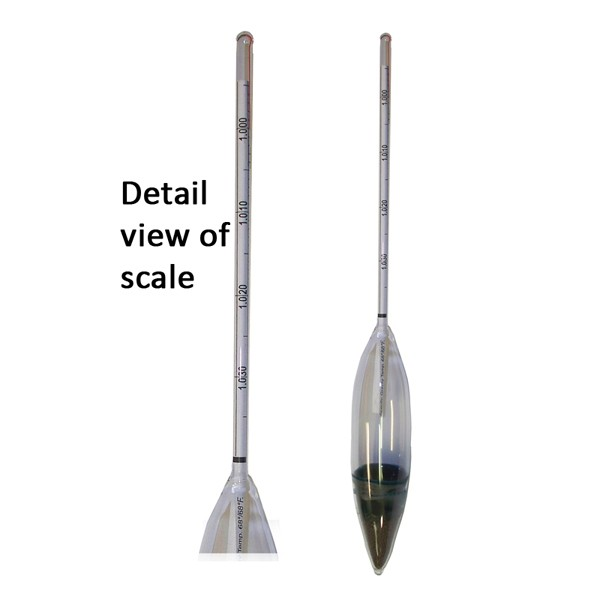
\includegraphics{Hydrometer151H.jpg}
	\caption{Hydrometer 151H. The specific gravity (relative density) of a liquid can be measured using a hydrometer. Hydrometers consist of a bulb attached to a stalk of constant cross-sectional area, as shown in the diagram to the right. The stalk of the hydrometer is pre-marked with graduations to facilitate measurement of the soil suspension, via Archimedes Principle.}
	\label{fig:Hydrometer151H}
\end{marginfigure}

Since the floating hydrometer is in static equilibrium, the downward gravitational force acting upon it must exactly balance the upward buoyancy force. The gravitational force acting on the hydrometer is simply its weight, mg. From the Archimedes buoyancy principle, the buoyancy force acting on the hydrometer is equal to the weight of liquid displaced. This weight is equal to the mass of liquid displaced multiplied by $\rho_\mathrm{ref}$ and the acceleration due to gravity. Thus, the force, $V\rho_{ref}$g\, where V is volume of displaced water, $\rho_{ref}$ is the density of the reference fluid, usually water:  $mg = V\rho_\mathrm{ref}g$, or by canceling the g, 

\begin{equation}\label{eq:massdisplaced}
m = \rho_\mathrm{ref} V,
\end{equation}

and as we'll see below, this can be rearranged to \sidenote{not rearranged... needs to be fixed}

\begin{equation}\label{eq:archmidies}
m = \rho_\mathrm{ref} V,
\end{equation}

Let's describe a comparison of two separate fluids to begin with as shown in Figure \ref{fig:Hydro}, where we can measure the displacement of they hydrometer's depth, where we can evaluate the differences in the relative densities: 

\begin{equation}
RD_{new/ref} = \rho_{new}/\rho{ref}
\end{equation}

\noindent where $\rho_{ref}$ is the known density (mass per unit volume) of the reference liquid (typically water);
$\rho_{new}$ is the unknown density of the new (green) liquid;
$RD_{new/ref}$ is the relative density of the new liquid with respect to the reference;

As the hydrometer is then suspended in a liquid of unknown density, $\rho_{new}$, as shown in green in Figure \ref{fig:Hydro}, where the change in displacement, $\Delta$x, is noted. In the example depicted, the hydrometer has dropped slightly in the green liquid; hence its density is lower than that of the reference liquid. It is, of course, necessary that the hydrometer floats in both liquids. In accordance with the way in which hydrometers are usually graduated, $\Delta$x is here taken to be negative if the displacement line rises on the stalk of the hydrometer, and positive if it falls. In the example depicted, $\Delta$x is negative.

\begin{marginfigure}
		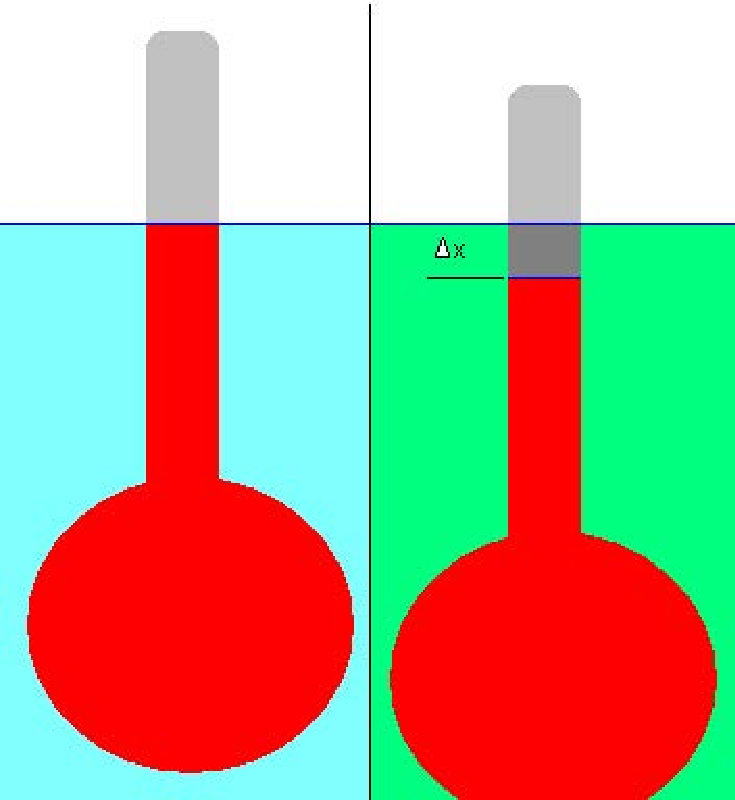
\includegraphics{Hydro.pdf}
	\caption{How does a hydrometer work? First the hydrometer is floated in the reference liquid (shown in light blue), and the displacement (the level of the liquid on the stalk) is marked (blue line). The reference could be any liquid, but in practice it is usually water. }
	\label{fig:Hydro}
\end{marginfigure}

We can modify Equation \ref{eq:archmidies}, by noting that the volume (V) displaced (the red in the figure) has been changed by the displaced volume A$\Delta$x, where A is the cross sectional area of the shaft. Thus, the mass of the hydrometer is 

\begin{equation}\label{eq:hydrometer}
m = \rho_\mathrm{new} (V - A \Delta x),
\end{equation}

\noindent By combining \ref{eq:massdisplaced} and \ref{eq:hydrometer}, we obtain

\begin{equation}\label{eq:RD1}
RD_{\mathrm{new/ref}} = \frac{\rho_\mathrm{new}}{\rho_\mathrm{ref}} = \frac{V}{V - A \Delta x}
\end{equation}

\noindent By re-arranging Equation \ref{eq:massdisplaced}, $V = m/\rho_{ref}$. We can substitute $m/\rho_\mathrm{ref}$ for V into into Eq. \ref{eq:RD1}:

\begin{equation}\label{eq:RD2}
RD_{\mathrm{new/ref}} = \frac{\rho_\mathrm{new}}{\rho_\mathrm{ref}} = \frac{m/\rho_\mathrm{ref}}{m/\rho_\mathrm{ref} - A \Delta x} = \frac{1}{1 - \frac{A \Delta x}{m} \rho_\mathrm{ref}}
\end{equation}

This equation allows the relative density to be calculated from the change in displacement, the known density of the reference liquid, and the known properties of the hydrometer. If $\Delta$x is small then, as a first-order approximation of the geometric series equation \ref{eq:RD2} can be written as:

\begin{equation}\label{eq:RD3}
RD_\mathrm{new/ref} \approx 1 + \frac{A \Delta x}{m} \rho_\mathrm{ref}
\end{equation}

Finally, Equation \ref{eq:RD3} describes how small $\Delta$x, changes in displacement, are approximately proportional to changes in relative density.

%\subsection{Calibrating a Hydrometer -- to be developed}

%Letting $\rho_s$ represent the suspension density, $\rho_f$ the density of fluid, and $\rho_{particle}$ the particle density, all in grams per liter, we have the equation, $\rho_s = \rho_f + (c/1000)(1 - \rho_f/\rho_{particle})$.  Although the buoyant force on a hydrometer is determined directly by the suspension density, r, hydrometer scales can be calibrated in terms of c for particular values of $\rho_l$ and $\rho_s$.  The large size of hydrometer bulb necessary to give adequate sensitivity reduces the depth discrimination of the instrument, but this limitation can be overcome by a simple correction \citep{day1965particle}.

\subsection{ASTM 422D Standard Test Method -- Hydrometer}

The methods to analyze particle distribution has been codified -- in what are compiled by ASTM International -- methods. In this case, the ASTM method 422D, Bouyoucos hydrometer method, was written to analyze particle size in soils or texture \citep{standard2007d422}. The Bouyoucos hydrometer method is somewhat less accurate than the pipet method, but is easier to perform.  The theory of the hydrometer method is similar to that of the pipet method except for the manner of determining the concentration of solids in suspension.  

For the hydrometer reading, the equation for particle size is relative to the effective depth of the hydrometer, in contrast to the distance that particles flow, where

$18 h = 30 l$

$l = 18h/30 = 0.6h$ or $h = 30l/18 = 1.67l$. Unfortunately, I have found no description of how this conversation has been calculated from first principles. For the 151H the effective depth is calculated as $l = 16.295 - 0.2645* R_c$,

However, the method makes a big deal of converting the Hydrometer reading, $R_c$ to the effective depth, that is used in Equation \ref{eq:effectivedepth}.

\begin{equation}\label{eq:effectivedepth}
\texttt{Effective Depth} = 16.295 - 0.1645*Rm
\end{equation}

For analysis of the particle distribution, we calculate the diameter of the particles that remain in suspension, where $d_t < d_0$,  

\begin{equation}
d_e = \sqrt{\frac{30 \eta l}{980 (GS_p - GS_f)* t}}
\end{equation}

\noindent where $d_e$ is the \emph{effective} or \emph{equivalent} settling diameter in mm, 
$\eta$ is the fluid viscosity,
l is effective depth,
$GS_p$ is the specific gravity of soil particles,
$GS_f$ is the specific gravity of fluid, and
$t$ is time of the observation.

In addition, we calculate the proportion of the particles that remain in suspension, which is often called \% Finer, or PF. In other words, the percentage of soil remaining in suspect at the level at which the hydrometer is measuring the density of the suspension may be calculated as follows:

\begin{equation}
PF = [(100,000/M_s)[m|5]P5 \frac{GS_p}{GS_p - GS_w}](R_c - GS_w)
\end{equation}

\noindent where $M_s$ is the soil weight and $GS_p$ is the ratio of the density of soil particles to the density of a reference substance; equivalently, it is the ratio of the mass of a substance to the mass of a reference substance for the same given volume. And $GS_w$ is the specific gravity of water.\sidenote{According to D422-63, using the value of one is appropriate.} $R_c$ is the hydrometer reading after the composite correction applied.\sidenote{The parameter $[m|5]P5$ is note described in the method -- so at this point, I am ignoring the term, which leaves one with an uncomfortable feeling.}

%\subsection{ASTM XXX Standard Test Method -- Pipet }

\subsection{Correction Factors to Consider}

The following are parameters that might influence the results of the hydrometer test and thus, we use various methods to pre-treat soils or measure to correct for these sources of bias. When correction factors are required, the calculations can become confusing.	 But we'll try to lead ourselves through this thicket without too many wrong-turns. 

\begin{description}
	\item[Temperature and Viscosity] Water temperate influences the viscosity of water, such that colder temperatures increase viscosity which increases the resistance force and reduces the terminal velocity of particles. The viscosity can be corrected for temperature.
	\item[Temperature and Density] The density of water is highest at 4.94 degrees C. As temperatures increases, the density of water decreases. As water density decreases, the suspension density $\rho_s$ decreases, thus the particle size distribution is not accurate without a correction. 
	\item[Soil Weight and Hygroscopic Water] Soil is composed of many components, including minerals, water, organic matter, air, etc. But to calculate the soil particle analysis, we need to account for the water in soil. We can do this by measuring the soil moisture content and correct the mass contributed by water from the soil tested.
	\item[Aggregated Soil Particles] Soil particles need to be dispersed, but there is no perfect way to accomplish this. Complete dispersion requires both mechanical and chemical assistance. Mechanical stirring overcomes weaker binding forces in large aggregates, but chemical agents are also necessary, especially to deflocculate clays. Polyvalent cations (normally \ce{Ca+2} and \ce{Al+3}) flocculate clays by forming interparticle, electrostatic links. Chemical dispersing agents (such as sodium hexametaphosphate) are effective in dispersing these clay bundles because:
	
	\begin{itemize}
		\item The sodium monovalent cation (\ce{Na+}) replaces polyvalent cations adsorbed on clays, breaking the interparticle linkage. The displaced polyvalent cations form insoluble complexes with phosphorus that prevents re-establishment of floccules.
		\item The adsorption of sodium, a highly hydrated cation, inducing the hydration of clays. This condition diminishes the binding strength between clay and cation which raises a clay particle's electronegativity and, hence, their repulsion from other clays.
	\end{itemize}
	
The mixture of dispersed soil particles in water is called a suspension. Once a true suspension state has been achieved, differential settling rates can be used to distinguish particle size distribution.
	
	\item Hydrometers are designed to be read from the bottom of the meniscus. However, in a soil suspension, the water is cloudy and we it's impossible to see through the meniscus. Therefore, we read the scale at the top of the meniscus and apply a correction factor. Without this correction factor, the analysis will be incorrect. 
\end{description}

\section{A Simplified Example}

It's generally tough to sort out scientific methods if you can't figure out what the end goal is. For this section, I am giving you an example of some calculations that might be done after the data have been collected.


\subsection{Determining Soil Amount}

After collecting and homogenizing the soil, we allow the soil to air-dry. Then, we passed the sample through the No. 10 sieve, what passes through the No. 10 sieve is particles less than 2 mm. This is considered soil, the rest are gravel or larger rocks. After weighing the percentage of soil that passed through the sieve, we calculated the percent passing through. 

When we report the data, we need to report it as a function of oven-dried soil. However, we don't want to used oven-dried soil for the sedimentation process. Thus, we need to know the difference between the oven-dried and air-dried soil. If the soil is mostly sand, we will need about 100 grams of oven-dried soil and if the soil is a silt or clay soil, we will only need 50 grams of oven-dried soil. 

Again, since we use air-dried soil, we have to correct for the moisture in the soil and use more soil than the 100 or 50 grams as specified above. We figured out that 53.3 grams of air-dried soil equals 50 grams of oven-dried soil, so our sample will have 53.3 grams of air-dried soil, but will be calculated as 50 grams.

\subsection{Observed Results}


We then weighed out 53.3 grams of air-dried soil and let it soak in sodium hexametaphosphate over night. Then we put the soil in 1000 l cylinders and vigorously mix the sample. We started the timer as we stopped mixing and took hydrometer and temperature readings at pre-selected times. 

Using a simple approach where the suspension density is measured several times after mixing, we might observe the following values:

% latex table generated in R 3.3.1 by xtable 1.8-2 package
% Thu Aug 18 07:56:06 2016
\begin{table}[ht]
\centering
\begin{tabular}{rrr}
  \hline
Elapsed Time & Hydrometer Reading & Temperature \\ 
  \hline
0.5 & 1.018 & 23 \\ 
  2.0 & 1.016 & 23 \\ 
  5.0 & 1.012 & 23 \\ 
  15.0 & 1.008 & 23 \\ 
  30.0 & 1.007 & 23 \\ 
  60.0 & 1.006 & 23 \\ 
  120.0 & 1.005 & 23 \\ 
  480.0 & 1.004 & 23 \\ 
  1440.0 & 1.003 & 23 \\ 
   \hline
\end{tabular}
\end{table}
\subsection{Calculating Particle Sizes}

\subsection{Simplest Calculation Method}

\begin{enumerate}
	\item (Clay + silt)\% = (($R_{40s}$ - $Rb_{40s}$)/$W_e$) x 100 
	\item Clay\% = (($R_{8h}$ - $Rb_{8h}$)/$W_e$) x 100 
	\item Silt\% = (Clay + silt)\% - Clay\%

	\item Sand\% = 100 -(($Rb_{40s}$ - $Rb_{40s}$) /$W_e$)*100
	\item Clay\% = ($R_{8h}$ - $Rb_{8h}$) / $W_e$)*100
	\item Silt\% = 100 - Sand\% - Clay\%

\noindent where $R_{40s}$ is the first hydrometer reading at 40s, 
$R_{8h}$ is the hydrometer reading at 8h,
$Rb_{40s}$ and $Rb_{8h}$ are the hydrometer reading of the blank cylinder without soil, and $W_e$ is the weight of soil in the cylinder.

	\item For temperature correction, add or subtract 0.36 g/L for each degree above or below 20$^\circ$C, respectively.
\end{enumerate}

\begin{Schunk}
\begin{Soutput}
[1] 0.074562997 0.037282114 0.023580057 0.013614402 0.009626915 0.006807313 0.004813537 0.002406788
[9] 0.001389571
\end{Soutput}
\begin{Soutput}
[1] 57.818182 51.393939 38.545455 25.696970 22.484848 19.272727 16.060606 12.848485  9.636364
\end{Soutput}
\end{Schunk}


\subsection{Classifying Soil Texture}

After determining the particle sizes, we can ``bin'' or categorize the particle sizes as percentages of sand, silt, and clay. 

\begin{figure}
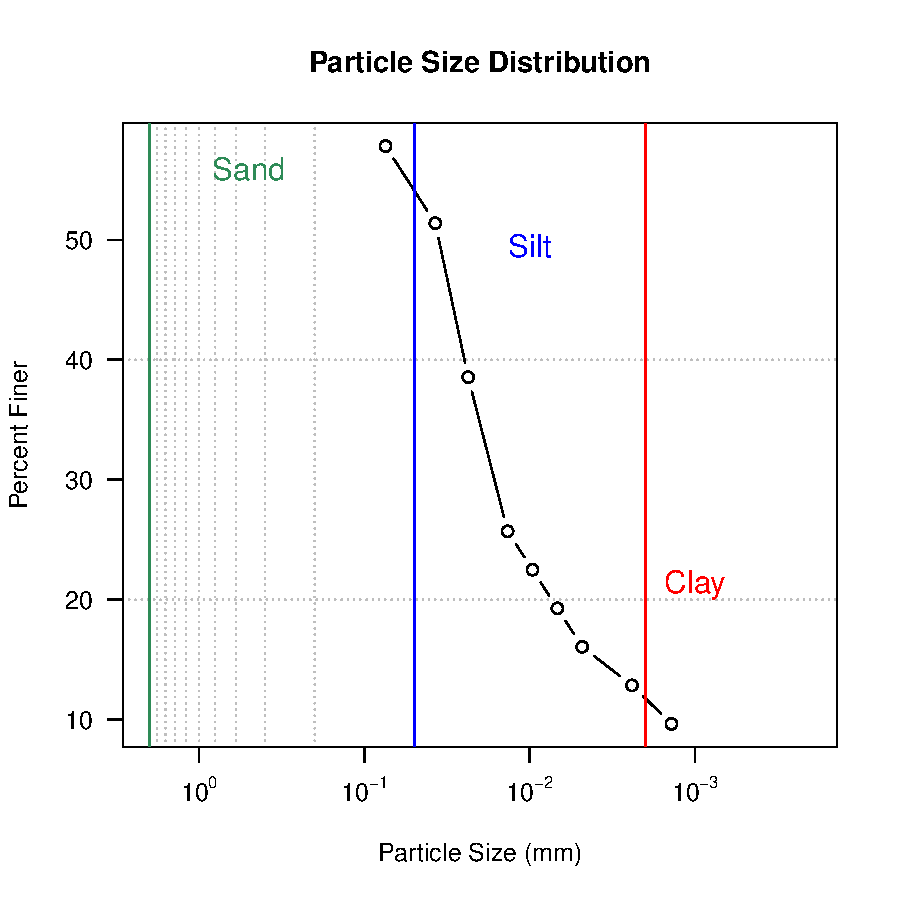
\includegraphics{Physics_Soil_Particle_Size_Analysis-simplifiedgraph}
\caption{Particle Size versus Percent Finer remaining in suspension.}
\label{fig.De_vs_PF}
\end{figure}

Using the figure, we estimated the following size classes. Obviously, it would be nice to do a better job than eye-balling the classes, but that will come later in the handout!

\begin{table}

		\begin{tabular}{lr}\hline
Size Class 	&		Percent		\\ \hline\hline
Sand				& 	55\% \\
Silt				&   33\% \\
Clay				& 	12\% \\ \hline		
		\end{tabular}
	\caption{Soil Texture -- Estimated from Figure \ref{fig.De_vs_PF}. Remember, these values should sum to 100\%!}
	\label{tab:SoilTexture}
\end{table}

Finally, we can determine what type of soil we have based on the size-class distribution, which is a sandy loam. 


\begin{figure*}
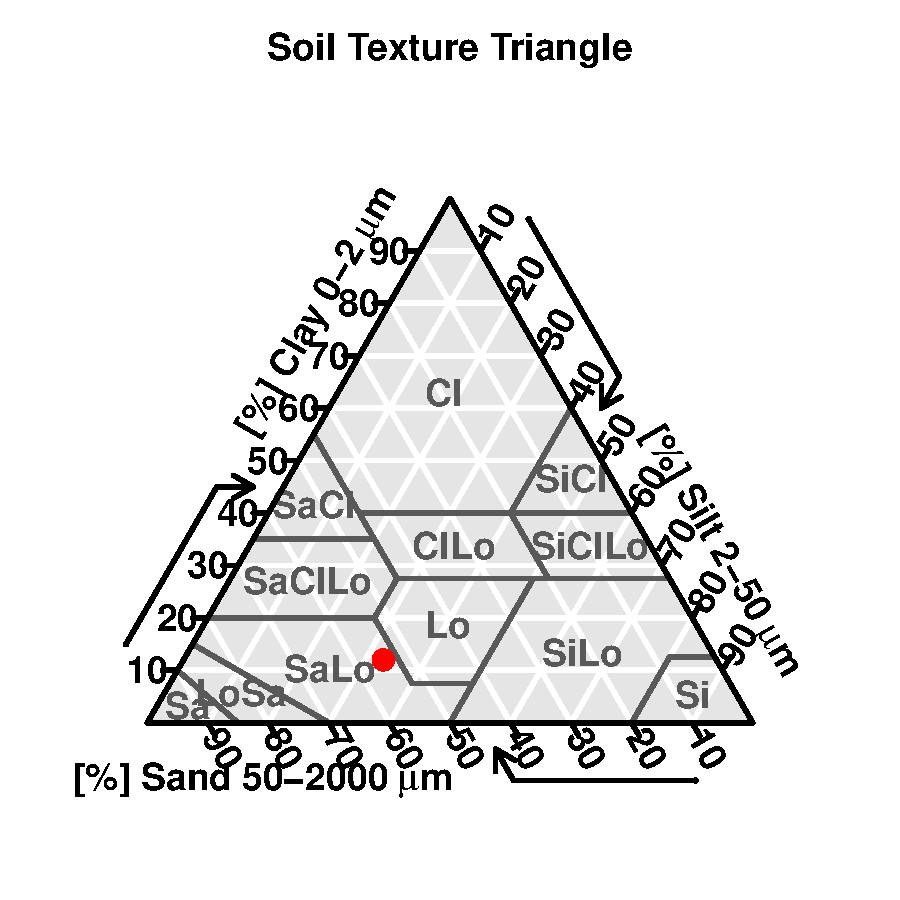
\includegraphics{Physics_Soil_Particle_Size_Analysis-TTPlot}
\caption{Results of our texture analysis. Note the small dot in the SaLo (sandy-loam) texture class.}
\label{fig.simplifiedfig}
\end{figure*}


\end{document}



